
\hypertarget{working_selectionmode}{}
\section{Selection mode}
\index{selection mode}

Allows the setting of the current selection mode
(Figure \ref{fig:selection_normal},
\ref{fig:selection_line} and
\ref{fig:selection_column}).

Select text by clicking and dragging with the left mouse button held
down or moving the cursor with the shift key held down. The status
bar will display an icon indicating the current selection mode.

\hypertarget{working_selectionmode_normal}{}
\subsection{Normal}
\index{selection mode!normal}

\begin{figure}[h!]
  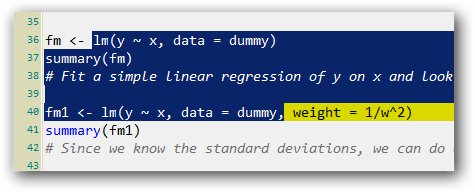
\includegraphics[scale=0.35]{./res/selection_normal.png}\\
  \caption{Normal (selection mode).}
  \label{fig:selection_normal}
\end{figure}

This is the standard selection mode
(Figure \ref{fig:selection_normal})
found in many Windows applications.

\hypertarget{working_selectionmode_line}{}
\subsection{Line}
\index{selection mode!line}

\begin{figure}[h!]
  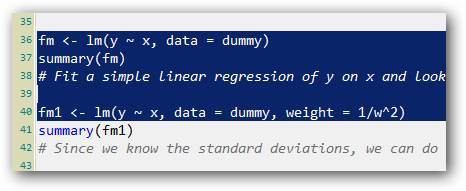
\includegraphics[scale=0.35]{./res/selection_line.png}\\
  \caption{Line (selection mode).}
  \label{fig:selection_line}
\end{figure}

This selection mode
(Figure \ref{fig:selection_line})
allows only for complete lines to be selected.

\hypertarget{working_selectionmode_column}{}
\subsection{Column}
\index{selection mode!column}

\begin{figure}[h!]
  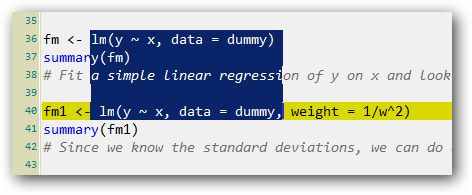
\includegraphics[scale=0.35]{./res/selection_column.png}\\
  \caption{Column (selection mode).}
  \label{fig:selection_column}
\end{figure}

This selection mode
(Figure \ref{fig:selection_column})
allows vertical blocks of text to be selected.
The option \texttt{ALT} sets column mode allowing the selection
mode to be switched to Column Mode when selecting with the mouse
by simply holding down the \texttt{ALT} key.
\htmladdnormallink{See details at editor (advanced options)}{\#working_editor_advanced}.
